\documentclass[onlytextwidth, aspectratio=169]{beamer}
\usepackage[utf8]{inputenc}
\usepackage{microtype}
\usepackage{amsmath}
\usepackage{amssymb}
\usepackage[nomessages]{fp} %\FPeval{\var-name}{2*sin(pi/6)}
\usepackage{siunitx} %units in math. eg 20\milli\meter
\usepackage{yhmath} % for arcs, overparenth command
\usepackage{tikz} %graphics
\usetikzlibrary{quotes, angles, arrows, arrows.meta}
%\usepackage{graphicx} already loaded by beamer class
%consider setting \graphicspath{{images/}}
%\parskip ?? to avoid paragraph indent
\usepackage{multicol} %may not need this package, just columns environment
\usepackage{venndiagram}

\subtitle[BECA]{Bronx Early College Academy}
\author[Huson]{Christopher J. Huson PhD}

\setbeamertemplate{headline}{\vskip2mm 
  \, BECA / \insertshortauthor \, / \inserttitle
  \hfill 
  \insertsection
  }

\title{Routines and Expectations: Assessment}
\date{2022-2023}

\begin{document}
\frame{\titlepage}

\section[Outline]{}
\frame{\tableofcontents}

\section{1.8 Assessment results, 28 September}
\begin{frame}{LT: How do we measure our efforts and results?}
  {CCSS: HSG.CO.A.1 Know precise geometric definitions  \hfill \alert{1.8 Wednesday 28 September}}
  \begin{block}{Do Now: Self-assessments questions}
  \begin{enumerate}
      \item How do we work efficiently and become a good scholar
      \item What should we know and be able to do
  \end{enumerate}
  \end{block}
  Jumprope, Mastery, Standards \\
  Exit Note Quiz
\end{frame}

\begin{frame}{Jumprope is our online system for grades}
  Use your @nycstudents.net login at https://www.jumpro.pe \\[0.25cm]
    Grades are from one to four \vspace{0.5cm}
    \begin{table}[ht]
      \textbf{Mastery Grades}
      \begin{tabular}[t]{p{0.20\linewidth} p{0.25\linewidth} p{0.18\linewidth} p{0.18\linewidth}}
        \hline
        1. Well below \newline expectations & 2. Approaching & 3. Meets & 4. Exceeds \\
        \hline
        Many missing or incorrect & Somewhat \newline correct & Detailed, \newline correct & Attempt \newline challenges \\[0.25cm]
        \hline
      \end{tabular}
    \end{table} \vspace{0.25cm}
\end{frame}

\begin{frame}{1.7 Exit Note Quiz \emph{standards}}
  {i.e. Skills or math topics, ``We hold ourselves to high standards''}
  \begin{block}{One grade in Jumprope for each}
      \begin{enumerate}
        \item {\tiny HSG.MG.A.1} Use geometric shapes, their measures, and their properties to describe objects \\[0.1cm]
          On problems 1 - 7 did you demonstrate mastery? \\
          (1: No, 2: Partly, 3: Largely) \\[0.2cm]
        \item {\tiny HSA.CED.A.1} Create equations in one variable and use them to solve problems. \\[0.1cm]
          Problem 8: $7x-12=3x$ \\
          (2: Incorrect, 3: Correct) \\[0.2cm]
        \item {\tiny 8.EE.C.7} Solve linear equations in one variable. \\[0.1cm]
          Problem 8: Solved as $x=3$ \\
          (2: Incorrect, 3: Correct)
        \end{enumerate}
      \end{block}
      \end{frame}

\begin{frame}{1.7 (Spicy) Extension Quiz, take home}
  {Challenge problems are for students who like to work hard in math and earn an \emph{A}}
  \begin{block}{{\tiny HSA.CED.A.1} \newline Create equations in one variable and use them to solve problems.}
      \begin{enumerate}
        \item Largely correct, score 4
        \item Somewhat correct, score 3 \\[0.2cm]
        Complete corrections to earn a 4 (required)
        \end{enumerate}
      \end{block} \vspace{0.5cm}
      \emph{Productive struggle} is key to learning \\[0.2cm]
      ``Struggling in mathematics is not the enemy any more than sweating is in basketball, it's a clear sign you are in the game.'' - Kim Sutton
      \vspace{1cm}
      \end{frame}

\begin{frame}{1.12 Unit Test: Mastery standards and criteria}
  {1: None, 2: Partly, 3: Largely (Earn a 4 by completing the spicy take-home test)}
      \begin{description}
        \item [\#1 - 3]{\tiny HSG.MG.A.1} Use geometric shapes, their measures, and their properties to describe objects \\[0.1cm]
          On problem 1, did you subtract to obtain length? \\[0.2cm]
          \item [\#4 - 8]{\tiny GPE.B.7} Compute perimeters and areas of triangles and rectangles. \\[0.1cm]
          Are the formulas in your notebook? (Notice especially that triangle area is $\frac{1}{2}$ of base times height)
          \item [\#9 - 11]{\tiny HSN.Q.A.3} Choose a level of accuracy appropriate to limitations on measurement when reporting quantities. \\[0.1cm]
          Can you find the formula for \% error in your notes?\\[0.1cm]
          \item [\#12 - 14]{\tiny HSA.CED.A.1} Create equations in one variable and use them to solve problems. \\[0.1cm]
          \#14 starts with: $(2x+4) + (x+3) = 22$
        \end{description}
      \end{frame}
      
\begin{frame}{Professionalism standard: Complete problem sets}
  {``Doing your work'' is how math skills and knowledge are developed.}
  Responsibility: Hands in assignments on time. Takes initiative to make up missing or absentee work. Meets deadlines and follows up when they are unable to meet a deadline. Is a positive model for academic success.

  %Completing assignments on time was cited by $83.1\%$ of students. \vspace{0.5cm}
    \begin{table}[ht]
      \textbf{Mastery Grade}
    \begin{tabular}[t]{p{0.25\linewidth} c c c }%{|p{2.4cm}|p{5.5cm}|p{8cm}|p{4cm}|}
      \hline
      1. Well below \newline expectations & 2. Approaching & 3. Meets & 4. Exceeds \\
      \hline
      \hspace{0.25cm} Minimal effort & Some work & Most work & Spicy \\[0.25cm]
      \hline
    \end{tabular}
  \end{table} \vspace{0.25cm}
    Satisfactory completion of an assignment requires \emph{effort}, but not perfection. (a score of $65\%$ is usually sufficient) Solutions are posted online. Check your answers and ask in class if you still do not understand.
    \vspace{1cm}
  \end{frame}

\begin{frame}{Professionalism: Taking notes}
  Writing mathematics helps you learn and gives you notes to study.\\[0.25cm]
    Students said taking notes in a notebook was the most important practice for successful learning $87.7\%$. \vspace{0.5cm}
    \begin{table}[ht]
      \textbf{Notebook Grade}
      \begin{tabular}[t]{p{0.25\linewidth} p{0.25\linewidth} p{0.15\linewidth} p{0.25\linewidth}}
        \hline
        1. Well below \newline expectations & 2. Approaching & 3. Meets & 4. Exceeds \\
        \hline
        Missing several notes & Largely complete & Detailed, \newline complete & Detailed, complete, neat \& organized \\[0.25cm]
        \multicolumn{4}{c}{1.6 Notebook ``treasure hunt''} \\[0.25cm]
        \hline
      \end{tabular}
    \end{table} \vspace{0.25cm}
\end{frame}

\begin{frame}{Notebook credit}
{Mastery grades 1 to 4}
\begin{block}{Take organized notes and study them for the test Friday}
    \begin{enumerate}
      \item Well below: Few notes or no notebook
      \item Approaching expectations: Many pages of notes in a composition book. Missing several formulas and definitions.
      \item Proficient: Well organized composition book with most or all formulas and terminology easy to locate.
      \item Extending: Assesses peers and gives constructive feedback.
      \end{enumerate}
    \end{block}
    \end{frame}

\begin{frame}{Professionalism assessment}
  {1: Well below, 2: Approaching, 3: Meets expectations, 4: Exceeds}
  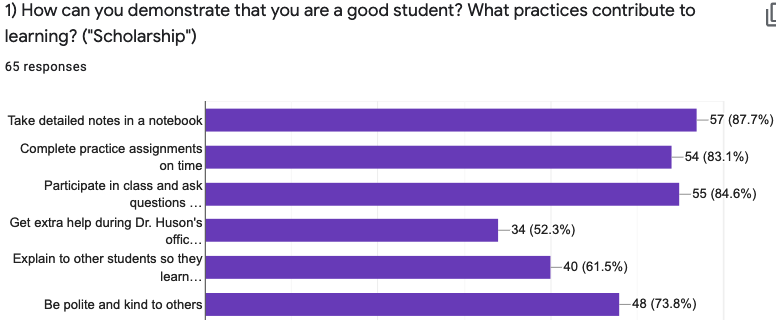
\includegraphics[width=.95\textwidth]{../graphics/scholarship-bar-chart.png}
  \begin{enumerate}
    \item Participate: Attendance (Google Classroom), Classkick
    \item Practice assignments: Khan Academy, Deltamath, 1.5 worksheet
    \item Detailed notes: Notebook treasure hunt uploads (weekend)
  \end{enumerate}
\end{frame}

\begin{frame}{What do I know, what can I do assessment}
  {1: Well below, 2: Approaching, 3: Meets expectations, 4: Exceeds}
  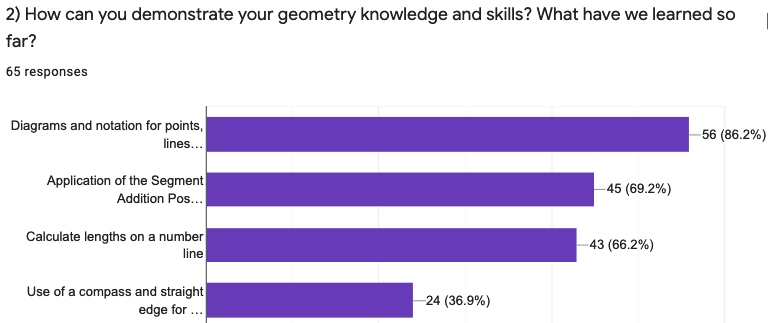
\includegraphics[width=.95\textwidth]{../graphics/know+do-bar-chart.png}
    \begin{enumerate}
      \item Classkick (open book, timed; use @beca324.org login):\\ Diagrams \& notation, segment addition, number line lengths
      \item Project: Construction of an equilateral triangle
    \end{enumerate}
  \end{frame}

\begin{frame}{Professionalism: Participation in class}
  Participation with classmates in the lessons conducted by the teacher is one of the primary inputs to learning.\\[0.25cm]
  Among Geometry students, $84.6\%$ considered it important. \vspace{0.5cm}
    \begin{table}[ht]
      \textbf{Participation Grade}
      \begin{tabular}[t]{p{0.25\linewidth} c c c }%{|p{2.4cm}|p{5.5cm}|p{8cm}|p{4cm}|}
        \hline
        1. Well below \newline expectations & 2. Approaching & 3. Meets & 4. Exceeds \\
        \hline
        \hspace{0.5cm}$<75\%$ & 75+\% & 100\% &  \\[0.25cm]
        \multicolumn{4}{c}{based on 11 assignments in Google Classroom (no late penalty)} \\[0.25cm]
        \hline
      \end{tabular}
  \end{table} \vspace{0.25cm}
  You must also load Genuis Scan and register in \emph{Classkick} as a portfolio user, or lose one level
  \vspace{1cm}
\end{frame}

  \end{document}